\section{Results}
\subsection{Testing setup and Evaluation}\label{testing_setup}

The tests are performed on a flat plane. This shape is chosen due to observing that the local area under the robot, when moving on a ship-hull resembles a plain with a slight amount of curvature. The flat test plane measures $100x42~meters$. 
The tests are made with 6 different initial starting poses. Then repeat thrice for each pose, resulting in 18 tests for each algorithm on each hull-shape. Each test was run for 180 \textit{(in simulation)} minutes, as testing showed this produced representable results while lessening the computations needed.

The robots position and orientation is sampled at 50 $Hz$, measured in meters with $2$ significant digits, with an attached timestamp. These data-points are evaluated for the \textit{coverage-over-time} and for coverage overlap.

The algorithms using beacon localization has been implemented with a pose estimation error of $5.2\%$, resulting in an error of $1.02~meters$ in the x and z direction and $0.51~meters$ in the y direction, relative to the world frame seen in figure \ref{fig:example_test_world}. This is done  assuming a minimum distance to the beacons of $20~meters$.\cite{beacon_error}

Each of these tests were then conducted multiple times and the mean and standard deviation were compared against the other algorithms in figure \ref{fig:results_graph}.
All the algorithms were tested by simulation for $180~minutes$. Table \ref{tab:res} shows the coverage that each algorithm reaches in this time-frame.
\subsection{Experimental Results}
The experiments was conducted according to section~\ref{testing_setup}.
The testings results from each algorithm is plotted in figure \ref{fig:results_graph}. This figure compares the average coverage of each algorithm over time. As such the most effective algorithm can be seen to be the \textit{\textbf{BBA}} with the horizontal path.

\begin{figure}[H]
    \captionsetup{justification=centering}
    \centering
    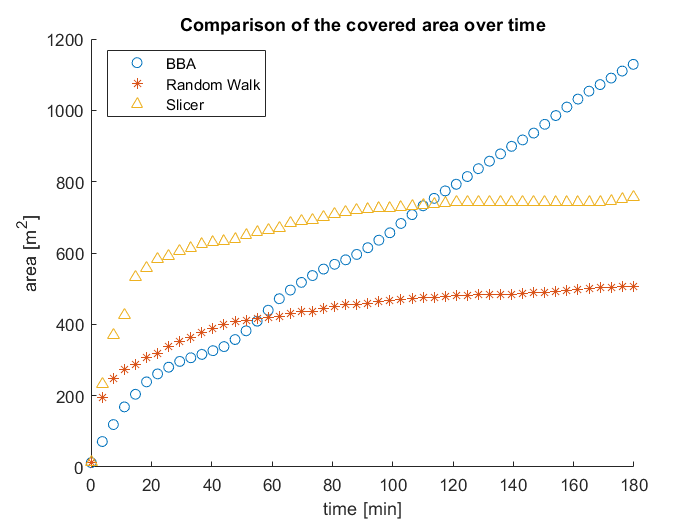
\includegraphics[width=0.5\textwidth]{Figures/comparison/oneArea.png}
    \caption{A graphical comparison of the navigation functions coverage in percentage over 3 hours in simulation.}
    \label{fig:results_graph}
\end{figure}
\begin{table}[H]
\begin{adjustbox}{max width=0.5\textwidth, center }
    \centering
    \begin{tabular}{|p{1.7cm}||p{1cm}|p{2cm}|p{1.5cm}|}
    \hline
    \multicolumn{4}{|c|}{Algorithm test} \\
    \hline
    Algorithm & Coverage in \%  & Coverage-over-time (180 min) & Gradient of covered area \\
    \hline
    \hline
    Random walk & 12\% & $506 m^2$ & $2.70~dm^2/ds$ \\
    Slicer & 18\%& $758 m^2$ & $4.03~dm^2/ds$ \\
    BBA & 27\% &$1129 m^2$ & $6.16~dm^2/ds$ \\
    \hline
    \end{tabular}
\end{adjustbox}
\captionsetup{justification=centering,margin=0cm}
\caption{Table of comparative results. The table data shows the efficiency results after 180 minutes in simulation.
}
\label{tab:res}
\end{table}

%SLOPES: BBA = 6.16; Random = 2.70; Slicer = 4.03
%std: BBA = 149.55 m^2; Random = 61.46 m^2; Slicer = 86.68 m^2

It was observed that the \textit{\textbf{BBA}} were more efficient over time after 120 minutes, compared to the \textbf{\textit{Slicer}} and the \textbf{\textit{Random Walk}} and had a higher efficiency until passing 60 min.
%\textcolor{red}{Algorithm A(add this when the we know what it is)}
The test results can be seen in figure~\ref{fig:results_graph}.

In figure \ref{fig:path}, the path followed by the \textit{\textbf{BBA}} (horizontal path) and the \textbf{\textit{Slicer}} (vertical path) are visualised, showcasing part of the established cleaning path due to the fact that the simulation times were up to $180 min$.

\begin{figure}[H]
    \captionsetup{justification=centering}
    \centering
    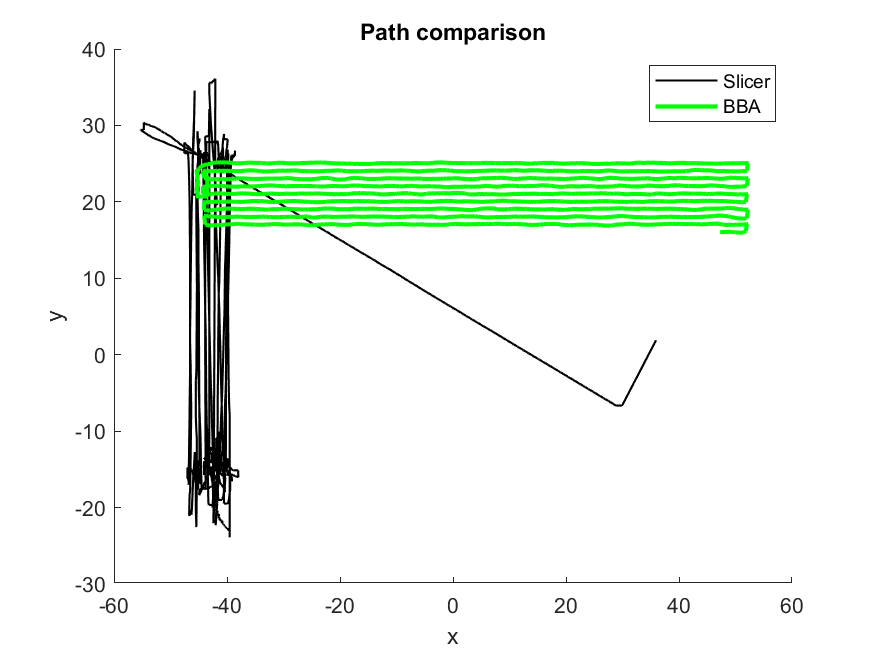
\includegraphics[width=0.5\textwidth]{Figures/comparison/path.png}
    \caption{A graphical comparison of the path followed by the Slicer and the BBA.}
    \label{fig:path}
\end{figure}